\RequirePackage{luatex85}
\documentclass{standalone}
\usepackage{tikz}
\usetikzlibrary{shapes.geometric}

% Color Definitions
\definecolor{SourceColor}{RGB}{85,168,104}
\definecolor{TargetColor}{RGB}{221,132,82}
\definecolor{TargetChangerColor}{RGB}{255,153,0}
\definecolor{AbsorbingAreaColor}{RGB}{196,78,82}
\definecolor{ObstacleColor}{RGB}{179,179,179}
\definecolor{StairColor}{RGB}{129,114,178}
\definecolor{MeasurementAreaColor}{RGB}{255,0,0}
\definecolor{AerosolCloudColor}{RGB}{202,156,76}
\definecolor{AgentColor}{RGB}{76,114,202}
\definecolor{AgentIdColor}{RGB}{255,127,0}

\newcommand{\MeasurementAreaOpacity}{0.549020}
\newcommand{\AerosolCloudOpacity}{0.039216}

\begin{document}
% Change scaling to [x=1mm,y=1mm] if TeX reports "Dimension too large".
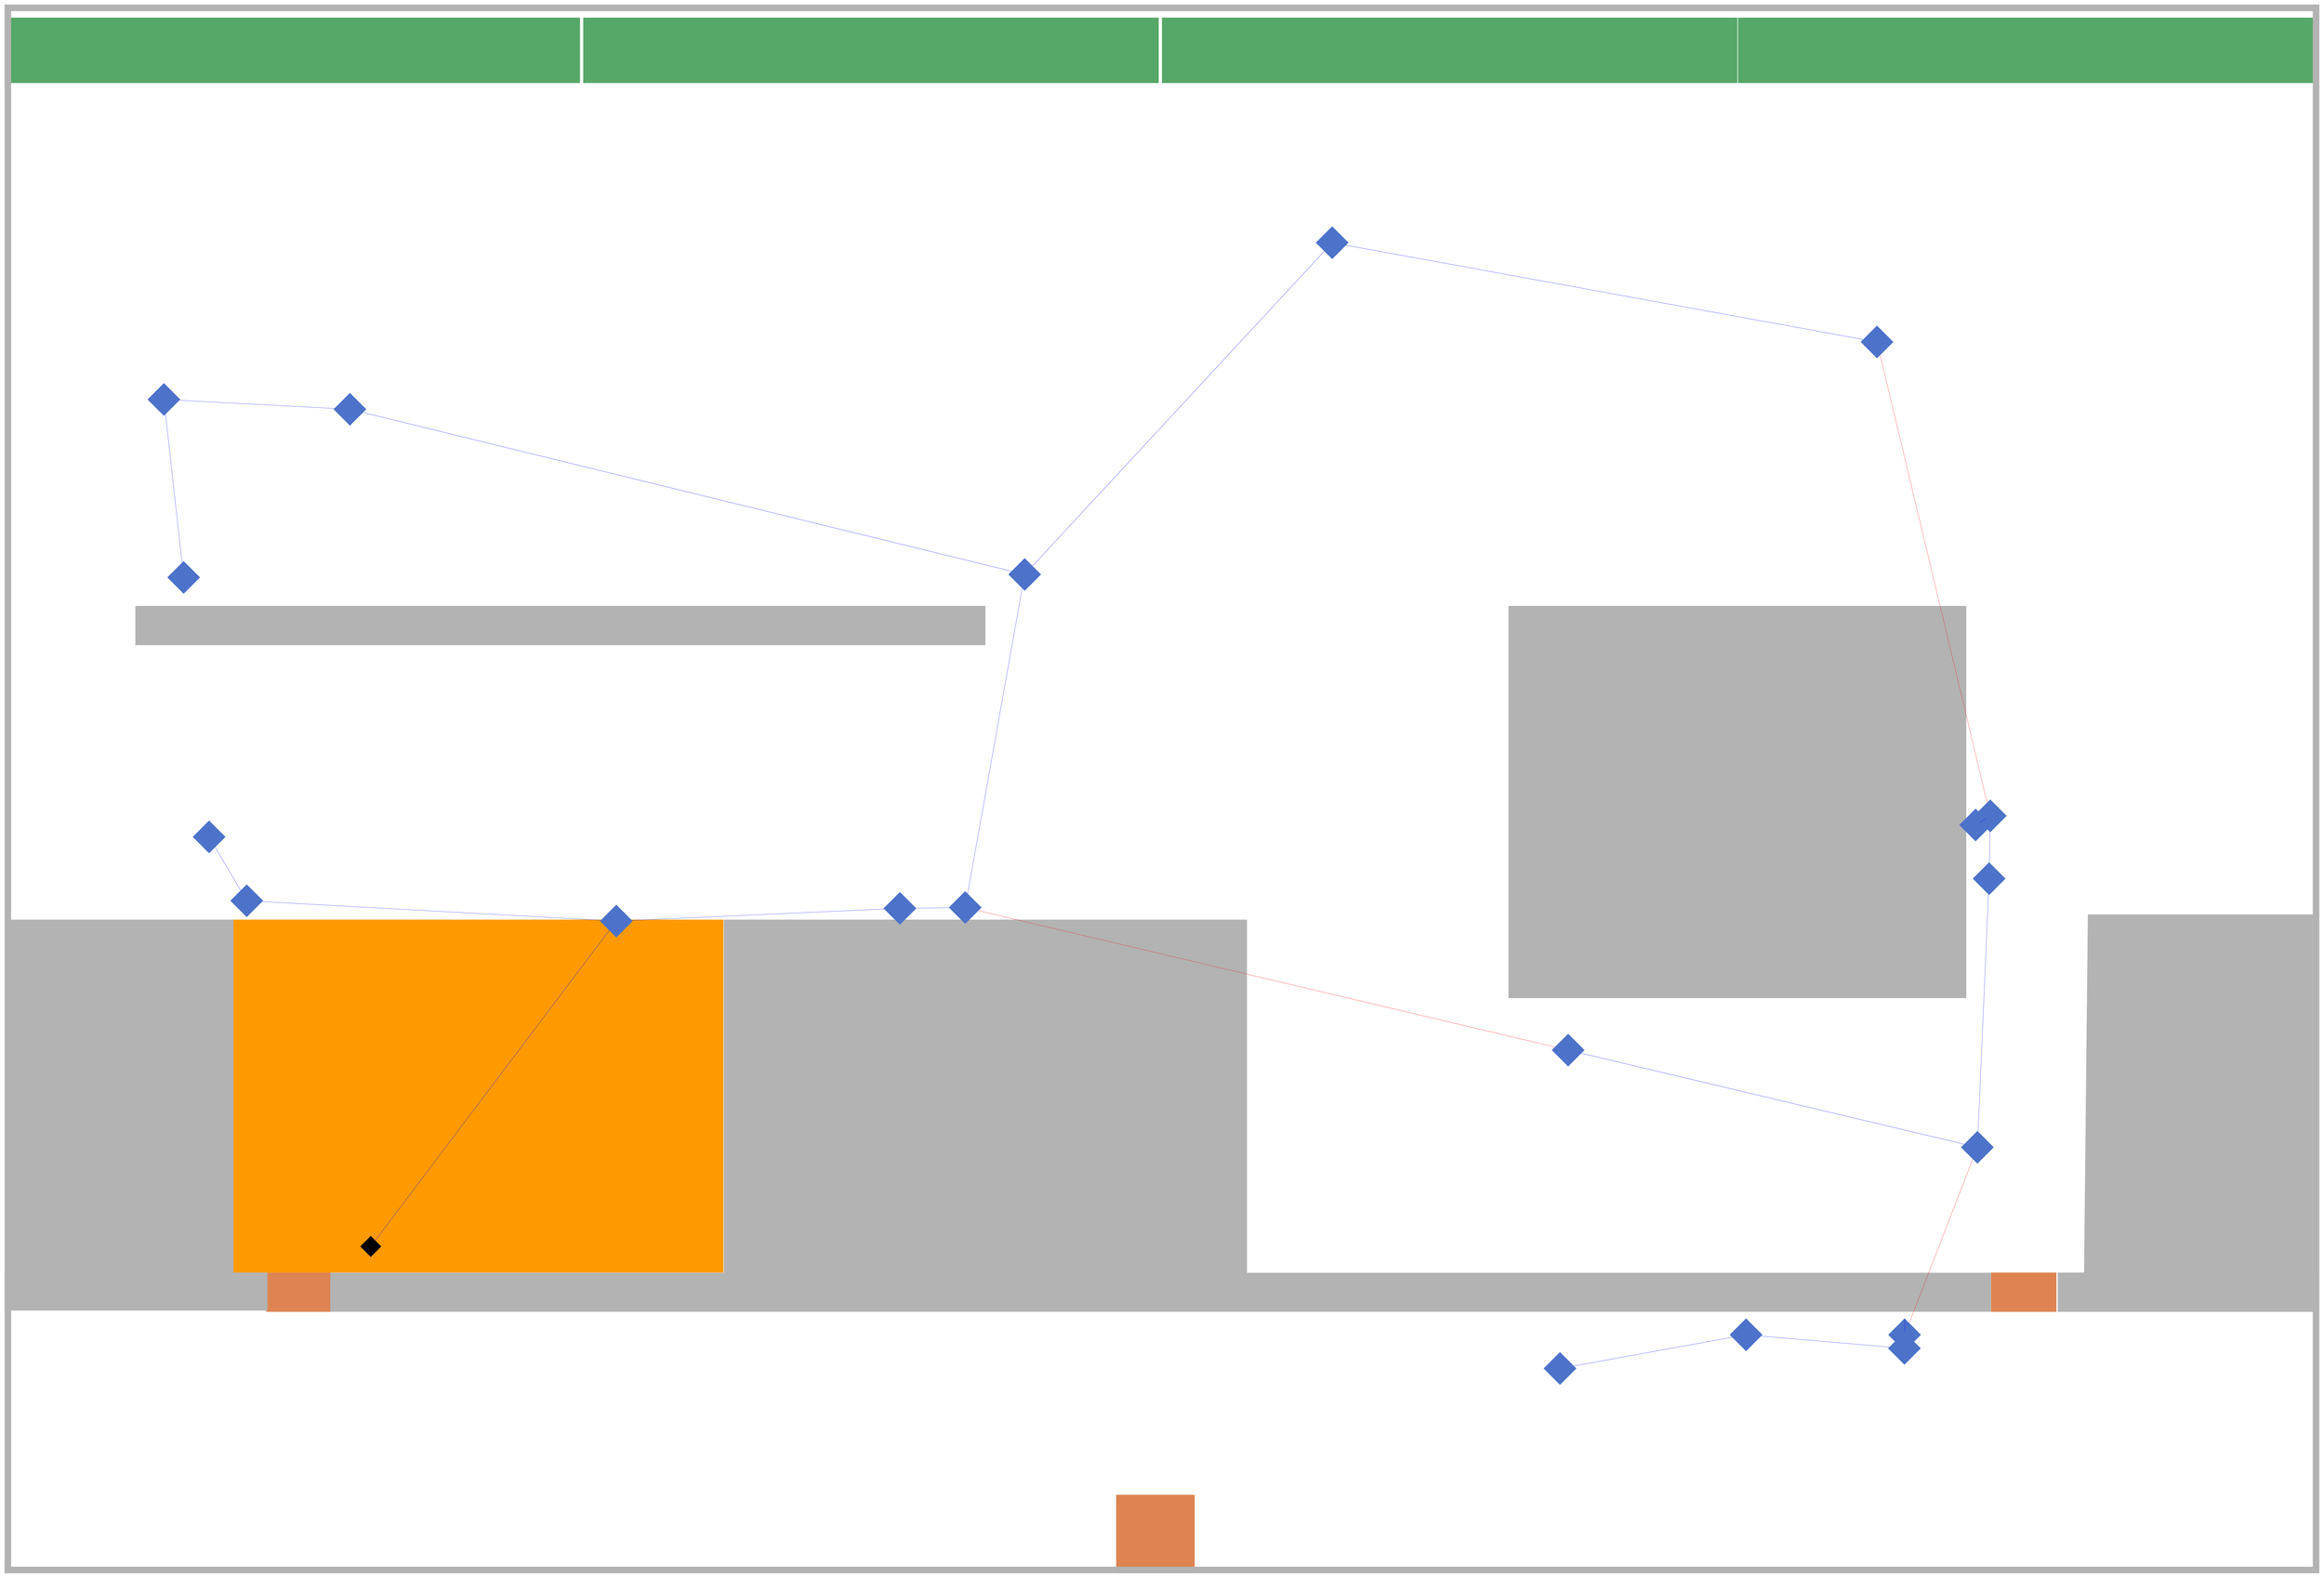
\begin{tikzpicture}
[x=1cm,y=1cm,
trajectory/.style={line width=1},
pedestrian/.style={diamond, fill=AgentColor, minimum size=2.5 cm},
walkdirection/.style={black, line width=1},
selected/.style={draw=magenta, line width=2},
group/.style={},
voronoi/.style={black, line width=1}
]

% Clipping
\clip (0.000000,0.000000) rectangle (177.000000,120.000000);
% Background
\fill[white] (0.000000,0.000000) rectangle (177.000000,120.000000);
% TargetChanger(s)
\coordinate (TargetChanger1) at (36.231244,36.500000); % Centroid: TargetChanger1
\fill[TargetChangerColor] (17.498110,23.000000) to (54.964378,23.000000) to (54.964378,50.000000) to (17.498110,50.000000) to (17.498110,23.000000);
% Source(s)
\coordinate (Source1) at (22.000000,116.500000); % Centroid: Source1
\fill[SourceColor] (0.000000,114.000000) to (44.000000,114.000000) to (44.000000,119.000000) to (0.000000,119.000000) to (0.000000,114.000000);
\coordinate (Source2) at (66.250000,116.500000); % Centroid: Source2
\fill[SourceColor] (44.250000,114.000000) to (88.250000,114.000000) to (88.250000,119.000000) to (44.250000,119.000000) to (44.250000,114.000000);
\coordinate (Source5) at (110.500000,116.500000); % Centroid: Source5
\fill[SourceColor] (88.500000,114.000000) to (132.500000,114.000000) to (132.500000,119.000000) to (88.500000,119.000000) to (88.500000,114.000000);
\coordinate (Source6) at (154.550000,116.500000); % Centroid: Source6
\fill[SourceColor] (132.550003,114.000000) to (176.550003,114.000000) to (176.550003,119.000000) to (132.550003,119.000000) to (132.550003,114.000000);
% Target(s)
\coordinate (Target2001) at (88.000000,3.000000); % Centroid: Target2001
\fill[TargetColor] (85.000000,0.000000) to (91.000000,0.000000) to (91.000000,6.000000) to (85.000000,6.000000) to (85.000000,0.000000);
\coordinate (Target2003) at (154.400000,21.500000); % Centroid: Target2003
\fill[TargetColor] (151.899994,20.000000) to (156.899994,20.000000) to (156.899994,23.000000) to (151.899994,23.000000) to (151.899994,20.000000);
\coordinate (Target2002) at (22.500000,21.500000); % Centroid: Target2002
\fill[TargetColor] (20.000000,20.000000) to (25.000000,20.000000) to (25.000000,23.000000) to (20.000000,23.000000) to (20.000000,20.000000);
% AbsorbingArea(s)
% Obstacle(s)
\coordinate (Obstacle12) at (132.500000,59.000000); % Centroid: Obstacle12
\fill[ObstacleColor] (115.000000,44.000000) to (150.000000,44.000000) to (150.000000,74.000000) to (115.000000,74.000000) to (115.000000,44.000000);
\coordinate (Obstacle13) at (42.500000,72.500000); % Centroid: Obstacle13
\fill[ObstacleColor] (10.000000,71.000000) to (75.000000,71.000000) to (75.000000,74.000000) to (10.000000,74.000000) to (10.000000,71.000000);
\coordinate (Obstacle5009) at (8.900000,35.800000); % Centroid: Obstacle5009
\fill[ObstacleColor] (17.500000,50.000000) to (0.300000,50.000000) to (0.300000,21.600000) to (17.500000,21.600000) to (17.500000,50.000000);
\coordinate (Obstacle2) at (9.850000,21.550000); % Centroid: Obstacle2
\fill[ObstacleColor] (-0.400000,20.100000) to (20.100000,20.100000) to (20.100000,23.000000) to (-0.400000,23.000000) to (-0.400000,20.100000);
\coordinate (Obstacle3) at (88.395264,21.497158); % Centroid: Obstacle3
\fill[ObstacleColor] (24.900000,20.007618) to (151.890518,20.007618) to (151.890518,22.986698) to (24.900000,22.986698) to (24.900000,20.007618);
\coordinate (Obstacle5002) at (75.000000,36.000000); % Centroid: Obstacle5002
\fill[ObstacleColor] (95.000000,50.000000) to (55.000000,50.000000) to (55.000000,22.000000) to (95.000000,22.000000) to (95.000000,50.000000);
\coordinate (Obstacle4) at (166.925928,21.500000); % Centroid: Obstacle4
\fill[ObstacleColor] (157.001205,20.000000) to (176.850647,20.000000) to (176.850647,23.000000) to (157.001205,23.000000) to (157.001205,20.000000);
\coordinate (Obstacle11) at (167.824784,36.159078); % Centroid: Obstacle11
\fill[ObstacleColor] (159.000000,22.000000) to (176.500000,22.000000) to (176.500000,50.400002) to (159.300003,50.400002) to (159.000000,22.000000);
% Aerosol Clouds
% Stairs
% Measurement Areas
\coordinate (MeasurementArea20) at (88.500000,60.000000); % Centroid: MeasurementArea 20
%\fill[MeasurementAreaColor,opacity=\MeasurementAreaOpacity] (0.500000,0.500000) to (176.500000,0.500000) to (176.500000,119.500000) to (0.500000,119.500000) to (0.500000,0.500000);
\coordinate (MeasurementArea10) at (88.700000,105.000000); % Centroid: MeasurementArea 10
%\fill[MeasurementAreaColor,opacity=\MeasurementAreaOpacity] (0.700000,90.000000) to (176.699997,90.000000) to (176.699997,120.000000) to (0.700000,120.000000) to (0.700000,90.000000);
% Voronoi Diagram (not enabled in config)
% Trajectories (not enabled in config)
% Agents
\node[pedestrian] (Pedestrian1) at (68.463109,50.864644) {};
\node[pedestrian] (Pedestrian2) at (119.559651,40.019886) {};
\node[pedestrian] (Pedestrian3) at (145.288057,18.240590) {};
\node[pedestrian] (Pedestrian4) at (118.936812,15.668402) {};
\node[pedestrian] (Pedestrian5) at (15.638386,56.328749) {};
\node[pedestrian] (Pedestrian6) at (18.516378,51.446435) {};
\node[pedestrian] (Pedestrian7) at (145.274430,17.204952) {};
\node[pedestrian] (Pedestrian8) at (133.166405,18.243733) {};
\node[pedestrian] (Pedestrian9) at (46.773056,49.890143) {};
\node[pedestrian] (Pedestrian10) at (73.455344,50.927774) {};
\node[pedestrian] (Pedestrian11) at (150.854096,32.584809) {};
\node[pedestrian] (Pedestrian12) at (150.717961,57.242474) {};
\node[pedestrian] (Pedestrian13) at (13.691682,76.179821) {};
\node[pedestrian] (Pedestrian14) at (26.406530,89.040968) {};
\node[pedestrian] (Pedestrian15) at (151.751561,53.135692) {};
\node[pedestrian] (Pedestrian16) at (151.838800,57.940248) {};
\node[pedestrian] (Pedestrian17) at (12.182802,89.790889) {};
\node[pedestrian] (Pedestrian18) at (78.001841,76.406481) {};
\node[pedestrian] (Pedestrian19) at (101.517115,101.784563) {};
\node[pedestrian] (Pedestrian20) at (143.176971,94.190587) {};
\node[pedestrian] (Pedestrian1) at (68.463109,50.864644) {};
\node[pedestrian] (Pedestrian2) at (119.559651,40.019886) {};
\node[pedestrian] (Pedestrian3) at (145.288057,18.240590) {};
\node[pedestrian] (Pedestrian4) at (118.936812,15.668402) {};
\node[pedestrian] (Pedestrian5) at (15.638386,56.328749) {};
\node[pedestrian] (Pedestrian6) at (18.516378,51.446435) {};
\node[pedestrian] (Pedestrian7) at (145.274430,17.204952) {};
\node[pedestrian] (Pedestrian8) at (133.166405,18.243733) {};
\node[pedestrian] (Pedestrian9) at (46.773056,49.890143) {};
\node[pedestrian] (Pedestrian10) at (73.455344,50.927774) {};
\node[pedestrian] (Pedestrian11) at (150.854096,32.584809) {};
\node[pedestrian] (Pedestrian12) at (150.717961,57.242474) {};
\node[pedestrian] (Pedestrian13) at (13.691682,76.179821) {};
\node[pedestrian] (Pedestrian14) at (26.406530,89.040968) {};
\node[pedestrian] (Pedestrian15) at (151.751561,53.135692) {};
\node[pedestrian] (Pedestrian16) at (151.838800,57.940248) {};
\node[pedestrian] (Pedestrian17) at (12.182802,89.790889) {};
\node[pedestrian] (Pedestrian18) at (78.001841,76.406481) {};
\node[pedestrian] (Pedestrian19) at (101.517115,101.784563) {};
\node[pedestrian] (Pedestrian20) at (143.176971,94.190587) {};
\node[draw, diamond, fill={rgb,255: red,0; green,0; blue,0}, minimum size=1.590000 cm] (sender)  at (28,25) {};
% Agent Ids (not enabled in config)
% Topography Boundary
\coordinate (TopographyBoundary1) at (88.500000,0.250000); % Centroid: TopographyBoundary -1
\fill[ObstacleColor] (-0.000100,0.500100) to (-0.000100,-0.000100) to (177.000107,-0.000100) to (177.000107,0.500100) to (-0.000100,0.500100);
\coordinate (TopographyBoundary2) at (176.750000,60.000000); % Centroid: TopographyBoundary -1
\fill[ObstacleColor] (176.499893,-0.000100) to (177.000107,-0.000100) to (177.000107,120.000099) to (176.499893,120.000099) to (176.499893,-0.000100);
\coordinate (TopographyBoundary3) at (88.500000,119.750000); % Centroid: TopographyBoundary -1
\fill[ObstacleColor] (177.000107,119.499901) to (177.000107,120.000099) to (-0.000100,120.000099) to (-0.000100,119.499901) to (177.000107,119.499901);
\coordinate (TopographyBoundary4) at (0.250000,60.000000); % Centroid: TopographyBoundary -1
\fill[ObstacleColor] (0.500100,120.000099) to (-0.000100,120.000099) to (-0.000100,-0.000100) to (0.500100,-0.000100) to (0.500100,120.000099);

\draw[red] (Pedestrian10) -- (Pedestrian2);
\draw[red] (Pedestrian20) -- (Pedestrian16);
\draw[red] (Pedestrian11) -- (Pedestrian3);



\draw[blue] (Pedestrian12) -- (Pedestrian16);
\draw[blue] (Pedestrian16) -- (Pedestrian15);
\draw[blue] (Pedestrian15) -- (Pedestrian11);
\draw[blue] (Pedestrian11) -- (Pedestrian2);


\draw[blue] (Pedestrian3) -- (Pedestrian7);
\draw[blue] (Pedestrian7) -- (Pedestrian8);
\draw[blue] (Pedestrian8) -- (Pedestrian4);



\draw[blue] (Pedestrian10) -- (Pedestrian18);
\draw[blue] (Pedestrian18) -- (Pedestrian14);
\draw[blue] (Pedestrian14) -- (Pedestrian17);
\draw[blue] (Pedestrian17) -- (Pedestrian13);
\draw[blue] (Pedestrian19) -- (Pedestrian18);
\draw[blue] (Pedestrian20) -- (Pedestrian19);


%
\draw[blue] (Pedestrian10) -- (Pedestrian1);
\draw[blue] (Pedestrian1) -- (Pedestrian9);
\draw[blue] (Pedestrian9) -- (Pedestrian6);
%
\draw[blue] (Pedestrian6) -- (Pedestrian5);

\draw[blue] (sender) -- (Pedestrian9);



%\draw[black,dashed, line width=1cm] (60,0) -- ++(117,110);

\end{tikzpicture}
\end{document}
